\section{Case Study}\label{sec:case-study}

This section presents a real data analysis using the classic Galaxies recession–velocity measurements. We follow the same dataset choice as \citet{bak2021penalized} and organize the discussion in three parts: (i) data description and preprocessing, (ii) density fitting and variance estimation for the density itself, and (iii) inference for several statistical estimands via plug–in HAL–MLE and HAL–TMLE.

\subsection{Data and preprocessing}
We analyze the \emph{Galaxies} data (R package \texttt{MASS}; \citealp{venables2002modern}), consisting of velocities for $n=82$ galaxies in the Corona Borealis region measured from six conic sections of space \citep[][Table~1]{postman1986probes}. If galaxies are clustered, the velocity density is expected to exhibit three to seven modes that correspond to superclusters \citep{roeder1990density}. 

For the preprocessing, we apply a monotone affine rescaling of the observed velocities to $[0,1]$. Throughout the figures, the horizontal axis represents the velocity as a proportion of the speed of light $c$: $x\in[0,1]$ corresponds to $v/c$. 

\subsection{Density fit and variance estimation}
We fit the HAL–MLE density on the rescaled axis. The resulting fit captures all prominent modes and the troughs between them, reflecting the heterogeneous galaxy population. We estimate the standard errors for the density via a delta–method as in Section~\ref{density_sd_section} and construct the confidence intervals. We benchmark these standard errors against a nonparametric bootstrap. This is a visualization of how bootstrap results differ from the delta-method results on the same small dataset. However, the bootstrap is much more computationally expensive, and thus we do not recommend it for practical use at this point. The shape of the density is similar to \citet{bak2021penalized} even though the data is rescaled.

\begin{figure}[H]
    \centering
    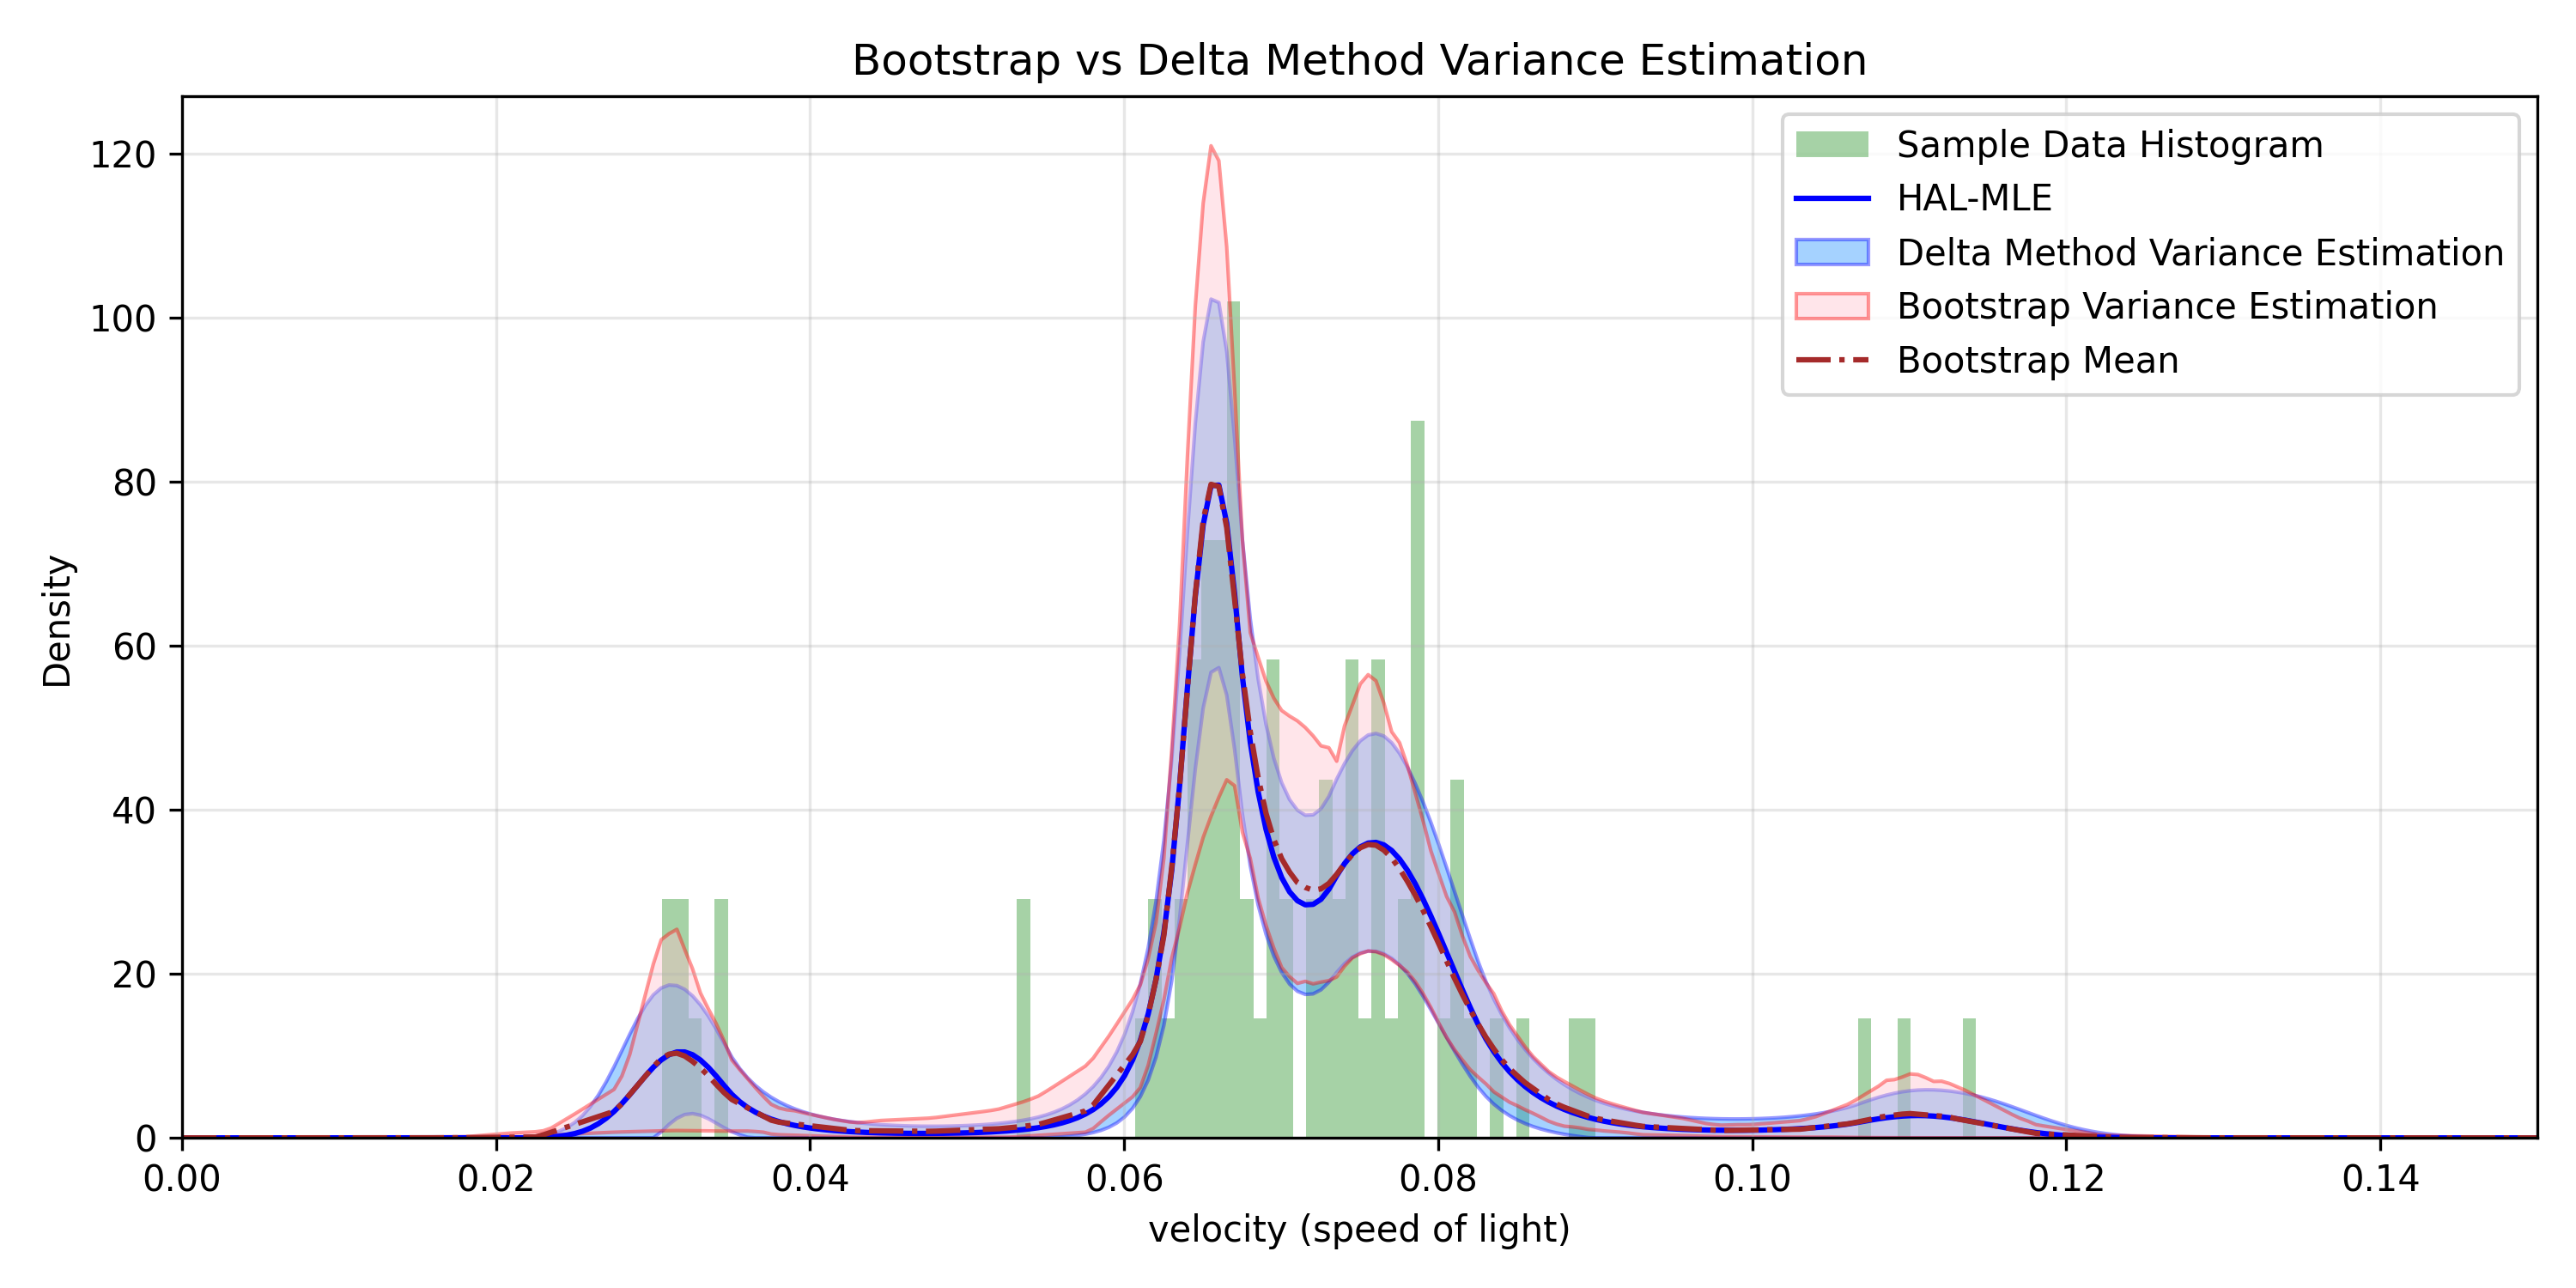
\includegraphics[width=\textwidth]{resources/case_study/bootstrap_vs_delta_method_variance_estimation.png}
    \caption{Galaxy velocities: histogram of the data with 50 bins, HAL–MLE density, and variance estimation for the density via the delta method (blue band) compared with a nonparametric bootstrap (red band).}
    \label{fig:galaxy-density-variance}
\end{figure}
Overall, the delta–method bands agree with the bootstrap, but there are regions where they are slightly narrower. One reason for this is that the parametric assumption of the Delta Method might cause under-estimation of variance. Another reason is that with the bootstrap, some bootstrap samples encounter the edge case of the solver, and the estimation is not accurate and varies a lot.

\subsection{Plug-in HAL-MLE versus HAL-TMLE}
We visualize the performance of the plug-in HAL-MLE and HAL-TMLE for the mean, median, and survival function. And we also visualize what targeting does to a fitted density based on the different statistical estimands. The results are shown below in Figure~\ref{fig:galaxy-mean}, Figure~\ref{fig:galaxy-median}, and Figure~\ref{fig:galaxy-survival}.

\begin{figure}[H]
    \centering
    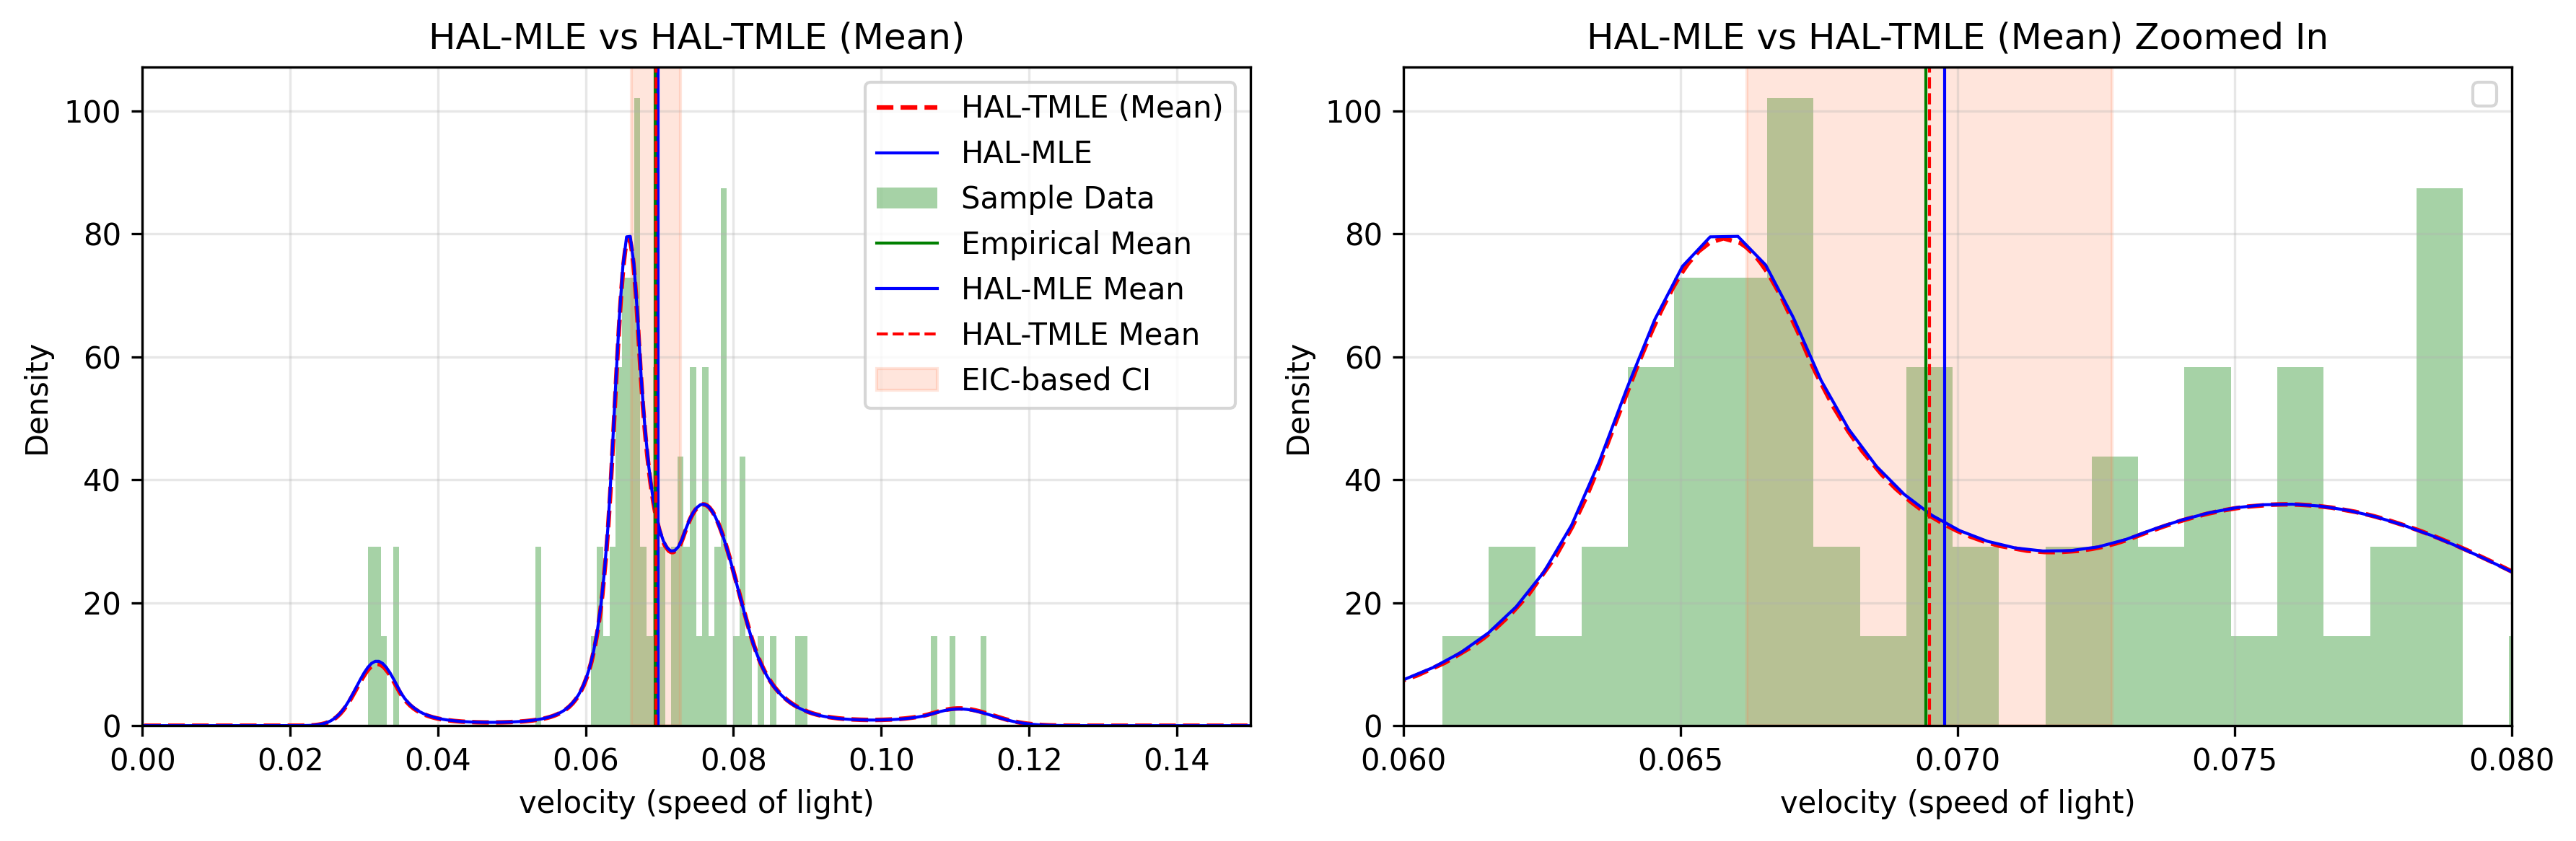
\includegraphics[width=0.9\textwidth]{resources/case_study/hal_mle_vs_hal_tmle_for_mean.png}
    \caption{Mean functional: plug–in HAL–MLE versus HAL–TMLE with the sample mean shown as the asymptotically efficient benchmark. Left: full scale; right: zoom around the dominant mode.}
    \label{fig:galaxy-mean}
\end{figure}

\begin{figure}[H]
    \centering
    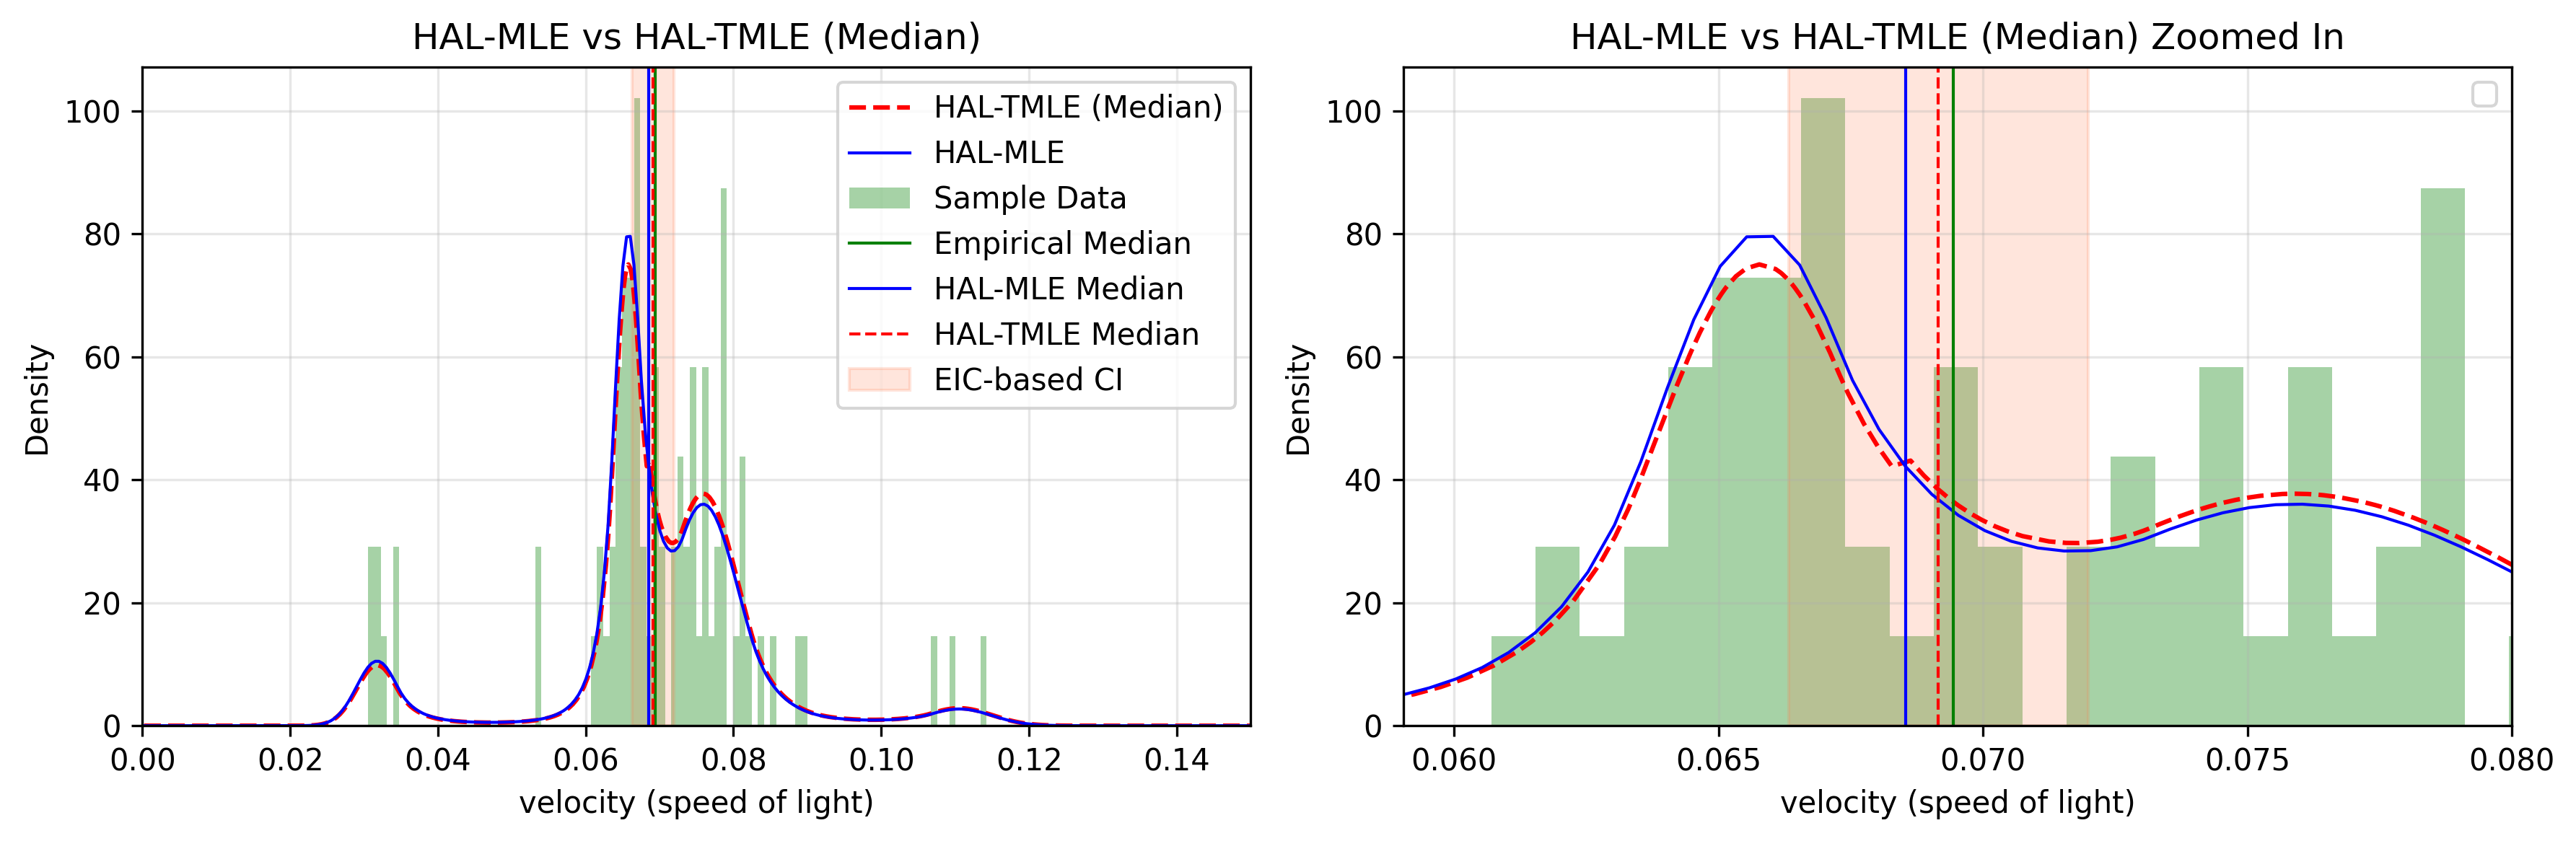
\includegraphics[width=0.9\textwidth]{resources/case_study/hal_mle_vs_hal_tmle_for_median.png}
    \caption{Median functional: plug–in HAL–MLE versus HAL–TMLE with the sample median shown for reference. Targeting nudges the estimate to align with the efficient score for the quantile.}
    \label{fig:galaxy-median}
\end{figure}

\begin{figure}[H]
    \centering
    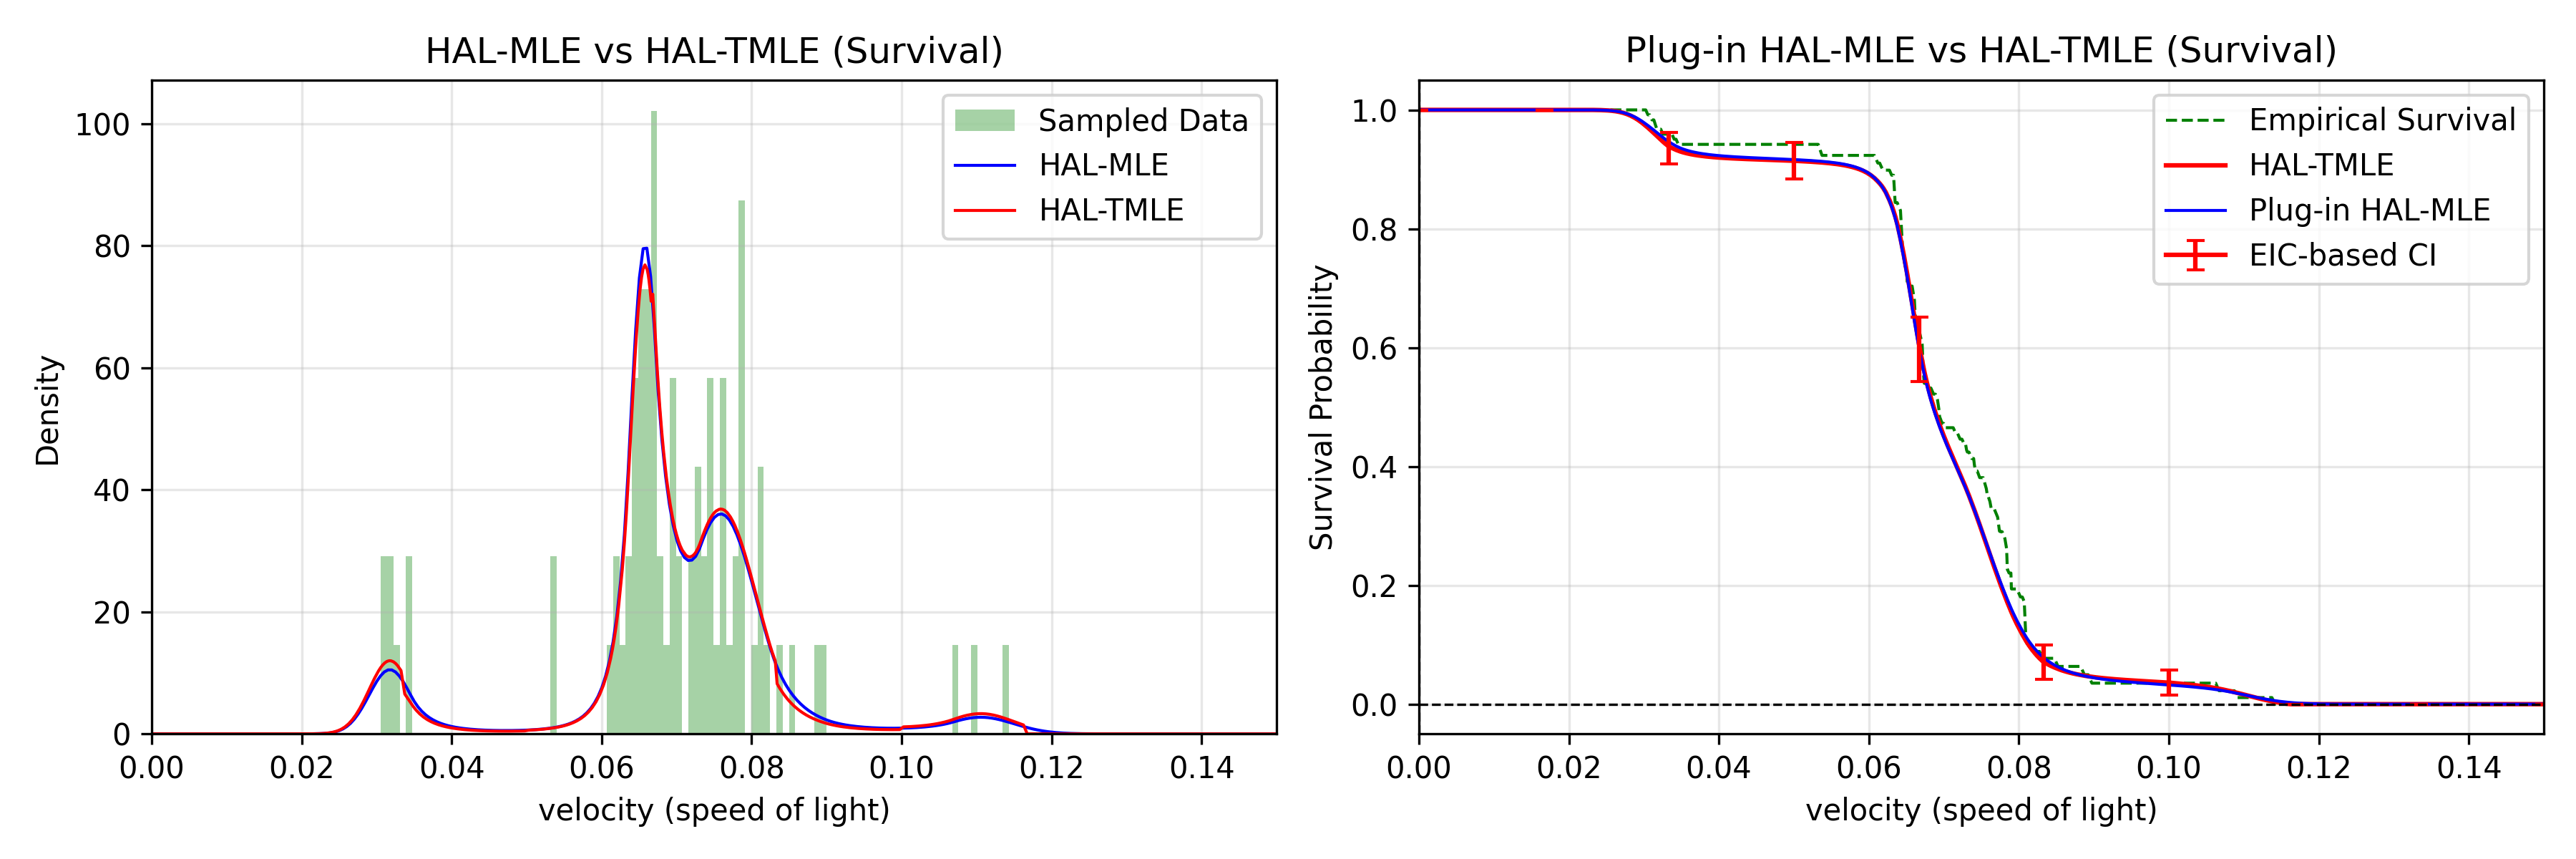
\includegraphics[width=0.9\textwidth]{resources/case_study/hal_mle_vs_hal_tmle_for_survival.png}
    \caption{Survival functional $S(t)$: plug–in HAL–MLE versus HAL–TMLE, compared to the empirical survival curve. Right panel overlays EIC–based intervals for representative $t$.}
    \label{fig:galaxy-survival}
\end{figure}

The TMLE of the survival function at 0.5 shifts the entire tail after 0.5 up and down. It solves the EIC equation, but it breaks the smoothness of the density. The TMLE of mean and median debiases the estimation from the plug-in HAL-MLE towards the sample mean and median, while still preserving a fitted density slightly different from the plug-in HAL-MLE.

